
%%%%%%%%%%%%%%%%%%%%%%%%%%%%%%%%%%%%%%%%%%%%%%%%%%%%%%%%%%%%%%%%%%%%%%%%
%Para las ecuaciones siempre es Ec.(n).
%Para las figuras siempre es Fig.n, incluso en el caption de la figura. Tambien las Tablas
%Para las referencias es [n]
%%%%%%%%%%%%%%%%%%%%%%%%%%%%%%%%%%%%%%%%%%%%%%%%%%%%%%%%%%%%%%%%%%%%%%%%

\documentclass[
reprint,
%notitlepage,
%superscriptaddress,
%groupedaddress,
%unsortedaddress,
%runinaddress,
%frontmatterverbose, 
%preprint,
%showpacs,preprintnumbers,
%nofootinbib,
%nobibnotes,
%bibnotes,
%11 pt,
amsmath,
amssymb,
aps,
%pra,
%prb,
%rmp,
%tightenlines %esto hizo el milagro de sacar los espacios en blancos estocásticos (?)
 %prstab,
%prstper,
%floatfix,\textbf{}
]{revtex4-1} %Instalar primero para usarlo. Paquete malo.

%\documentclass[onecolumn, aps, amsmath,amssymb ]{article}
\usepackage{lipsum}  
\usepackage{graphicx}% Include figure files
\usepackage{subfig}
\usepackage{braket}
\usepackage{comment} %comment large chunks of text
\usepackage{dcolumn}% Align table columns on decimal point
\usepackage{bm}% bold math
%\usepackage{hyperref}% add hypertext capabilities
\usepackage[mathlines]{lineno}% Enable numbering of text and display math
%\linenumbers\relax % Commence numbering lines
\usepackage{mathtools} %% Para el supraíndice

\usepackage[nice]{nicefrac}

%%%%%%%El Señor Español%%%%%%%%%%%%%%%%%%%%%%%%%%%
\usepackage[utf8]{inputenc} %acento
\usepackage[
spanish, %El lenguaje.
es-tabla, %La tabla y no cuadro.
activeacute, %El acento.
es-nodecimaldot %Punto y no coma con separador de números
]{babel}
\usepackage{microtype} %para hacerlo más bonito :33 como vos (?) 
%%%%%%%%%%%%%%%%%%%%%%%%%%%%%%%%%%%%%%%%%%%%%%%%%%%
%%%%%%%%% Para que las imágenes se queden dónde las quiero (?
\usepackage{float}
%%%%%%%%%%

%%%%%%%%Cambia a Fig de Figure%%%%%%%%%%
\makeatletter
\renewcommand{\fnum@figure}{Fig. \thefigure} 
\makeatother
%%%%%%%%%%%%%%%%%%%%%%%%%%%%%%%%%%%%%%%%
\raggedbottom


\begin{document}
%%%%%%%%%%%%%%%%%%%%%%%%%%%%%%%%%%Título%%%%%%%%%%%%%%%%%%%%%%%%%%%%%%%%%%%%%%
%%%%%%%%%%%%%%%%%%%%%%%%%%%%%%%%%%%%%%%%%%%%%%%%%%%%%%%%%%%%%%%%%%%%%%%%%%%%%%

\title{Anisotropías para todos los disparos y pesos de los hexágonos}
\author{Evelyn~G.~Coronel}

\affiliation{
Tesis de Maestría en Ciencias Físicas\\ Instituto Balseiro\\}

\date[]{\lowercase{\today}} %%lw para lw, [] sin date

%\begin{abstract}

%\end{abstract} 
\maketitle
%%%%%%%%%%%%%%%%%%%%%%%%%%%%%%%%%%%%%%%%%%%%%%%%%%%%%%%%%%%%%%%%%%%%%%%%%%%%%%%%%%%
% Podemos usar cualquiera de los dos comandos: \input o \include para incluir el texto

%\subsubsection{Nomenclatura}
%
%	\begin{table}[H]
%	\centering
%		\begin{tabular}{c|c|c|c}
%	Archivo AllTriggers  & \text{Eventos} & UTC inicial &  UTC final  \\ \hline
%	2020			 & 13 739 351	  &  1372680068	&  1577879983 \\ %2019
%	2019			 & 	8 463 063	  &	 1372680068 &  1496318388 \\ %Herald
%	2017			 &	8 592 302	  &  1372680068 &  1498521517 \\ %Oscar
%			\end{tabular}
%			\end{table}
%



\section{Anisotropías  considerando el peso de los hexágonos}

\subsection{Variación de los pesos en función de la ascensión recta}
En las figuras de esta sección se muestran el análisis en ascensión recta para los eventos de observatorio considerando las variaciones de la exposición. 
Los mismos se hicieron en el mismo intervalo de tiempo para poder compararlos entre sí. Elegí el rango presentado en la Tabla \ref{rango_corto}  porque en el mismo se encuentran todos los eventos filtrados por energía, por bad period, por reconstrucción correcta, etc. El rango empieza en el 2013 porque la última versión del archivo de todos los disparos empezó a registrarse desde el  1 de Julio del 2013 a las 12:01:08 GMT (1372680068) hasta el  1 de enero del 2020 a las 11:59:43 (1577879983). Mientras que el archivo del disparo estándar va desde el 01 de enero del 2004.

	\begin{table}[H]
	\centering
		\begin{tabular}{c|c|c|c}
	 		& UTC 			& Fecha		 	&  Hora GMT  \\ \hline
	Inicio	& 1372699409	&2013-07-01 	&17:23:29		\\
	Final 	& 1577825634	&2019-12-31 	&20:53:54		\\
		\end{tabular}
	\caption{Rango de tiempo considerando todos los disparos} 	\label{rango_corto}
	\end{table}


Un ejemplo de como son los pesos para tres frecuencias en particular, en este rango de tiempo, se muestra en la Fig.\,\ref{fig:pesos}


\begin{figure}[H]
	\centering
	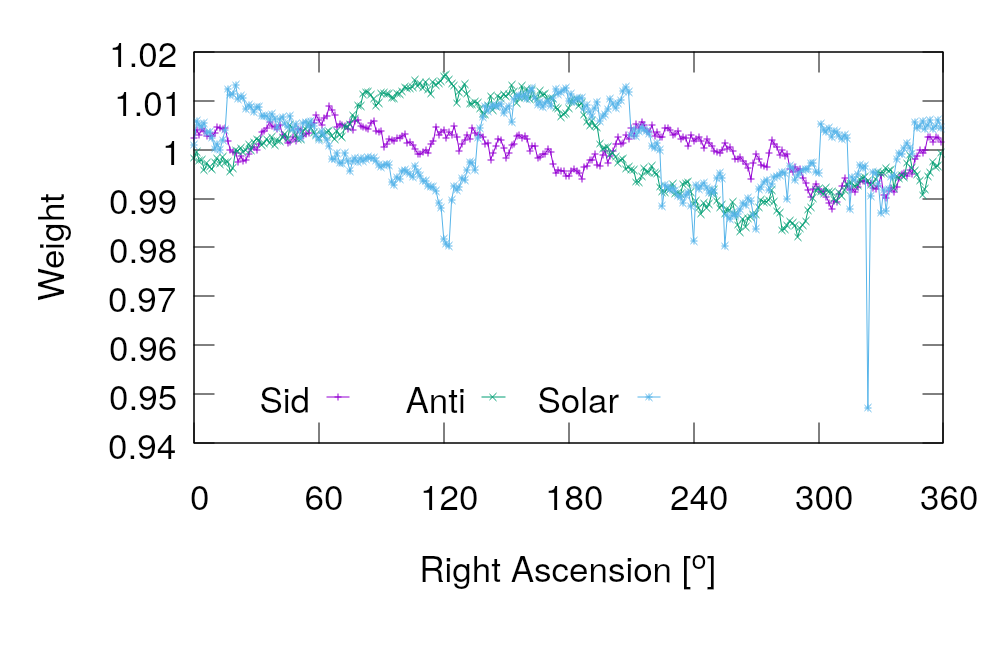
\includegraphics[width=0.5\textwidth]{pesos_side_sola_anti.png}
	\caption{Pesos para las frecuencias sidérea, solar y anti-sidérea}
	\label{fig:pesos}
\end{figure}


\subsubsection{Energía entre 1\,EeV y 2\,EeV}

Para este caso utilizamos el archivo con todos los disparos en el rango de energía $1\,$ EeV - $2\,$EeV donde se tiene $1\,321\,702$ eventos.

\begin{figure}[H]
	\centering
	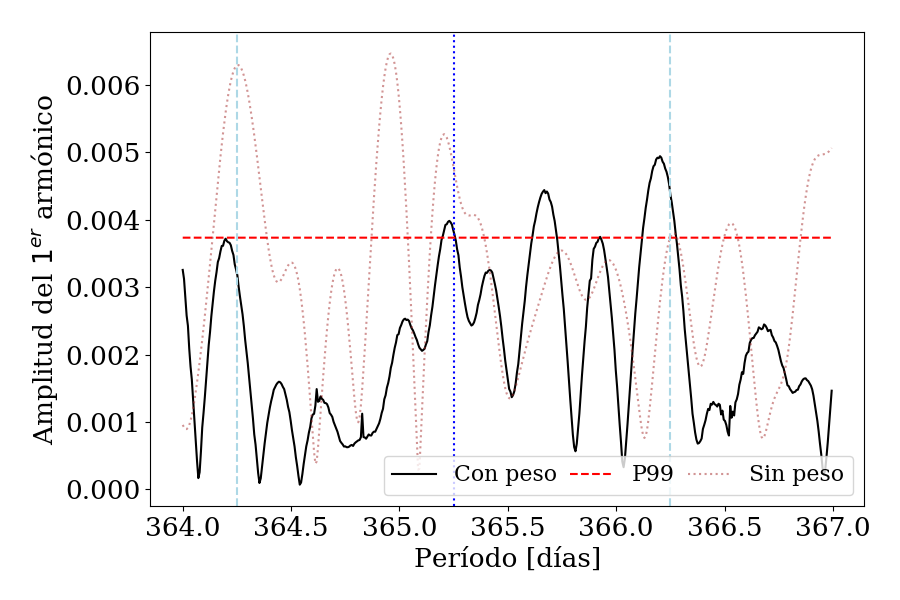
\includegraphics[width=0.5\textwidth]{2019_AllTriggers_1_2_EeV_con_vs_sin_peso.png}
	\caption{Todos los disparos: entre 1 EeV y 2 EeV}
	\label{fig:12w}
\end{figure}
%fig

\subsubsection{Energía entre 2\,EeV y 4\,EeV}

Para este caso utilizamos los eventos del archivo con todos los disparos con energía entre $2\,$ EeV - $4\,$EeV, donde se encontraron $288\,444$ eventos.
\begin{figure}[H]
	\centering
	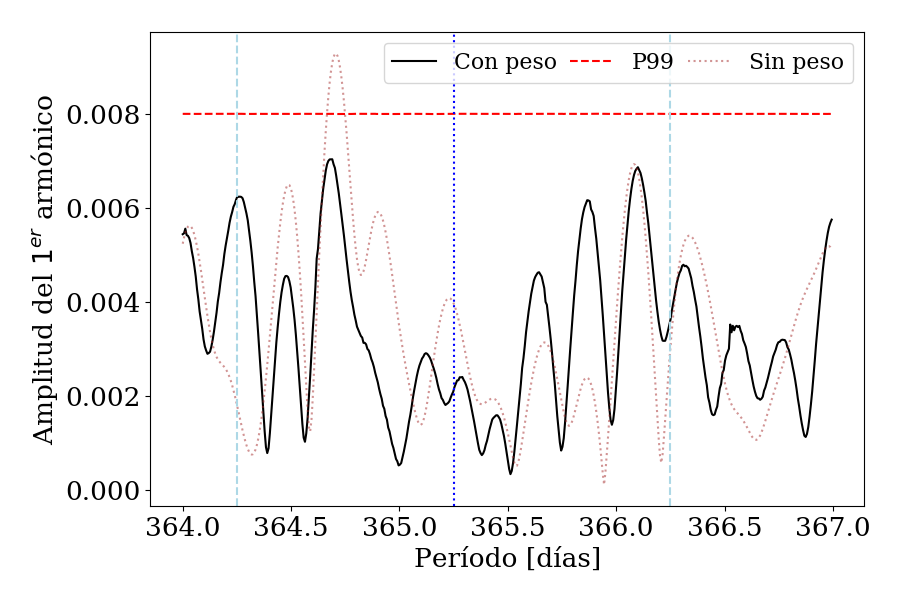
\includegraphics[width=0.5\textwidth]{2019_AllTriggers_2_4_EeV_con_vs_sin_peso.png}
	\caption{Todos los disparos: entre 1 EeV y 2 EeV}
	\label{fig:24w}
\end{figure}

En la Fig.\,\ref{fig:24w} no se ve ningún pico por encima de  percentil 99.


\subsubsection{Energía entre 4\,EeV y 8\,EeV}

A partir de $3\,$EeV el disparo estándar tiene una eficiencia del $100\%$. Entonces para este  intervalo de energías,  utilizamos el archivo con el disparo estandar.

\begin{figure}[H]
	\centering
	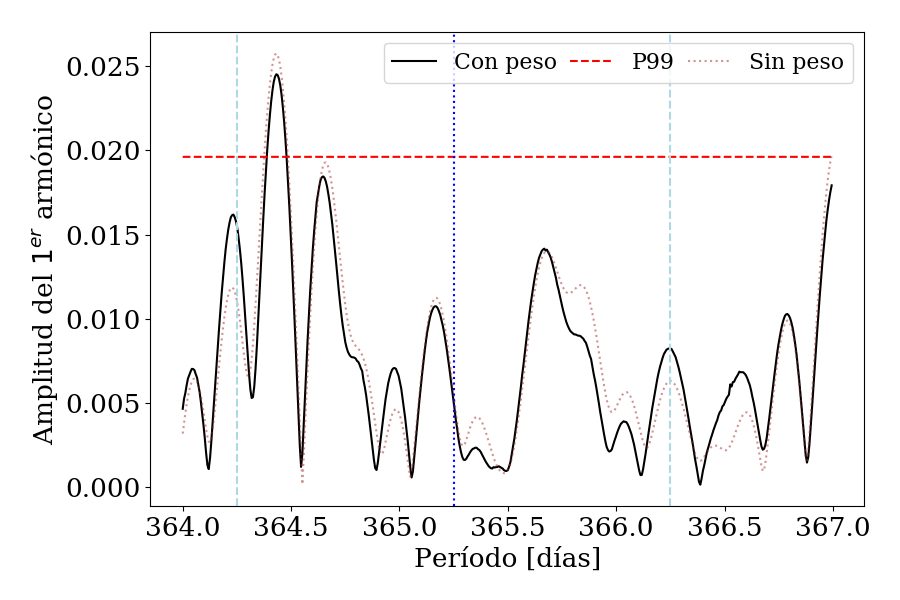
\includegraphics[width=0.5\textwidth]{2019_Main_Array_4_8_EeV_con_vs_sin_peso.png}
	\caption{Disparos estándar: entre 4 EeV y 8 EeV}
	\label{fig:48w}
\end{figure}
%fig

\subsubsection{Energía sobre 8\,EeV}

Para este caso utilizamos el archivo con el disparo estandar

\begin{figure}[H]
	\centering
	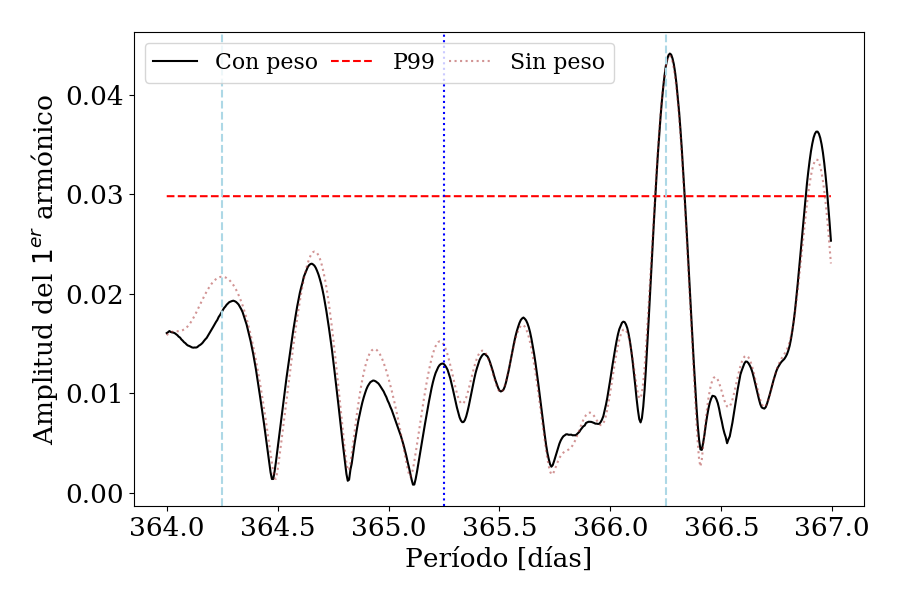
\includegraphics[width=0.5\textwidth]{2019_Main_Array_8_EeV_con_vs_sin_peso.png}
	\caption{Disparos estándar: entre 1 EeV y 2 EeV}
	\label{fig:48w}
\end{figure}
%fig




\subsection{Ampliando el rango de tiempo para el archivo del disparo estándar}

Amplié el rango de tiempo para poder compararlo con los gráficos anteriores, ya que se espera que mientras mayor sea el rango de tiempo
	\begin{table}[H]
	\centering
		\begin{tabular}{c|c|c|c}
	 		& UTC 			& Fecha		 	&  Hora GMT  \\ \hline
	Inicio	& 1104537600	&2005-01-01 	&00:00:00		\\
	Final 	& 1577825634	&2019-12-31 	&20:53:54		\\
		\end{tabular}
	\end{table}

\end{document}
